\documentclass[14pt]{extarticle}
\usepackage[utf8]{inputenc}
\usepackage[T1]{fontenc}
\usepackage[spanish,es-lcroman]{babel}
\usepackage{amsmath}
\usepackage{amsthm}
\usepackage{physics}
\usepackage{tikz}
\usepackage{float}
\usepackage{calc}
\usepackage[autostyle,spanish=mexican]{csquotes}
\usepackage[per-mode=symbol]{siunitx}
\usepackage{gensymb}
\usepackage{multicol}
\usepackage{enumitem}
\usepackage{setspace}
\usepackage[left=2.00cm, right=2.00cm, top=2.00cm, 
     bottom=2.00cm]{geometry}
\usepackage{Estilos/ColoresLatex}
\usepackage{makecell}
\usepackage{subcaption}

% \usepackage[sfdefault]{roboto}  %% Option 'sfdefault' only if the base font of the document is to be sans serif
% \usepackage[T1]{fontenc}

\usepackage{scalerel}[2016-12-29]
\def\stretchint#1{\vcenter{\hbox{\stretchto[440]{\displaystyle\int}{#1}}}}
\def\scaleint#1{\vcenter{\hbox{\scaleto[3ex]{\displaystyle\int}{#1}}}}
\def\bs{\mkern-12mu}

\newcommand{\textocolor}[2]{\textbf{\textcolor{#1}{#2}}}
\sisetup{per-mode=symbol}
\decimalpoint
\sisetup{bracket-numbers = false}
\newlength{\depthofsumsign}
\setlength{\depthofsumsign}{\depthof{$\sum$}}
\newcommand{\nsum}[1][1.4]{% only for \displaystyle
    \mathop{%
        \raisebox
            {-#1\depthofsumsign+1\depthofsumsign}
            {\scalebox
                {#1}
                {$\displaystyle\sum$}%
            }
    }
}

\title{\vspace*{-2cm} Interferencia}
\date{ }

\begin{document}
\maketitle

\section{Fenómenos de interferencia.}

La interferencia ocurre cuando dos ondas mutuamente coherentes se superponen en algún lugar del espacio. Como se vio en el capítulo anterior, estas ondas son mutuamente coherentes solamente en dos casos posibles:
\begin{enumerate}[label=\alph*)]
\item si tienen su origen en la misma fuente,
\item si son monocromáticas y tienen exactamente la misma frecuencia, como en el caso de algunos láseres.
\end{enumerate}
La superposición de dos ondas coherentes con la misma longitud de onda se discutió ampliamente en el capítulo anterior. Supongamos que dos ondas salen de una fuente luminosa y recorren caminos diferentes para después reunirse nuevamente en una pantalla. La fase de cada una de las ondas al llegar a la pantalla puede expresarse como:
\begin{align}
\theta = \scaleint{6ex}_{\bs 1}^{2} k \dd{x}
\label{eq:ecuacion_IX_01}
\end{align}
suponiendo que el índice de refracción $n$, y por lo tanto el valor de $k$, es función del punto $x$ de la trayectoria. Si ahora sustituimos el valor de $k$ dado por:
\begin{align}
k = n \, k_{0}
\label{eq:ecuacion_IX_02}
\end{align}
donde $k_{0}$ es el valor de $k$ en el vacío, y usamos la definición de camino óptico $CO$ dada en el primer capítulo, podemos obtener:
\begin{align}
\theta = k_{0} \, (CO)
\label{eq:ecuacion_IX_03}
\end{align}
Ahora, si una de las ondas recorre un camino óptico $CO_{1}$ y la otra recorre un camino óptico $CO_{2}$ de la fuente al punto de observación, las fases de ellas en este punto serán:
\begin{align}
\theta_{1} = k_{0} \, (CO_{1})
\label{eq:ecuacion_IX_04}
\end{align}
y
\begin{align}
\theta_{2} = k_{0} \, (CO_{2})
\label{eq:ecuacion_IX_05}
\end{align}
De aquí se ve que la diferencia de fase está dada por:
\begin{align}
\theta_{21} = \theta_{2} - \theta_{1} = k_{0} (DCO)
\label{eq:ecuacion_IX_06}
\end{align}
donde $DCO$ es la diferencia de camino óptico entre los dos haces. Por lo tanto, la irradiancia en el detector quedaría dada por:
\begin{align}
I = I_{1} + I_{2} + 2 \, \sqrt{I_{1} \, I_{2}} \, \cos \left[ k_{0} \, (DCO) \right]
\label{eq:ecuacion_IX_07}
\end{align}
donde $I_{1}$ e $I_{2}$ son las irradiancias de cada haz de manera independiente. Se puede ver que la máxima irradiancia se obtiene para valores de la diferencia de camino óptico dados por: 
\begin{align}
DCO = m \, \lambda
\label{eq:ecuacion_IX_08}
\end{align}
donde $m$ es un entero. La mínima amplitud, que es cero, se obtiene cuando:
\begin{align}
DCO = n \, \dfrac{\lambda}{2}
\label{eq:ecuacion_IX_09}
\end{align}
donde $n$ es un entero impar.

\subsection{Interferencia  de dos fuentes puntuales separadas.}

Como un ejemplo de interferencia, supongamos dos fuentes luminosas puntuales y perfectamente coherentes separadas por una pequeña distancia, como se muestra en la figura (\ref{fig:figura_IX_01}).
\begin{figure}[H]
    \centering
    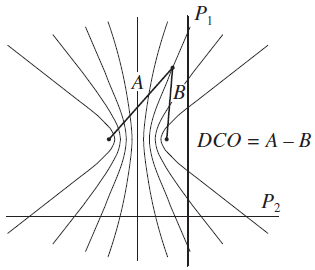
\includegraphics[scale=1]{Imagenes/Interferencia_01.png}
    \caption{Líneas que representan el lugar geométrico de los puntos con diferencia de camino óptico constante, con dos fuentes luminosas puntuales.}
    \label{fig:figura_IX_01}
\end{figure}
Los lugares en el espacio donde hay interferencia constructiva estarán en posiciones tales que:
\begin{align}
A - B = m \, \lambda
\label{eq:ecuacion_IX_10}
\end{align}
Como $A - B$ es una constante, los lugares geométricos de los puntos con interferencia constructiva serán hiperboloides de revolución, como se muestra en la figura (\ref{fig:figura_IX_01}). Si el plano de observación es perpendicular a la línea que une las dos fuentes, las franjas serán circulares. En cambio, si el plano es paralelo a esta línea, las franjas serán hipérbolas, las cuales se aproximan a franjas rectas y paralelas cerca del centro de la pantalla.

\section{Interferencia por división de frente de onda.}

Los dos haces luminosos que interfieren se pueden obtener a partir de un frente de onda, con cualquiera de los dos procedimientos siguientes:
\begin{enumerate}[label=\alph*)]
\item dividiendo lateralmente el frente de onda en dos, sin cambiar su irradiancia, y
\item separando el frente de onda en dos y dividiendo su irradiancia en dos, pero preservando su extensión lateral.
\end{enumerate}
La división de frente de onda se puede lograr por medio de difracción, reflexión o refracción, como se verá más adelante. En cualquier caso, la luz que ilumine el interferómetro debe ser espacialmente coherente.

\subsection{Doble rendija de Young.}

La división del frente de onda de que se ha hablado se puede efectuar de manera muy simple mediante una doble rendija, como se muestra en la figura (\ref{fig:figura_IX_02}).
\begin{figure}[H]
    \centering
    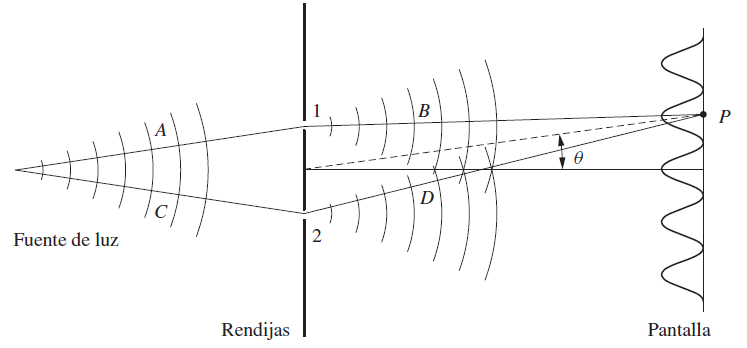
\includegraphics[scale=0.7]{Imagenes/Interferencia_02.png}
    \caption{Franjas de Young formadas con dos rendijas rectas y paralelas.}
    \label{fig:figura_IX_02}
\end{figure}
Al llegar el frente de onda a las rendijas, ésta se expande en forma angular en cada uno de los agujeros debido a un fenómeno llamado difracción, que se estudiará más adelante.

Las distancias de las rendijas $1$ y $2$ al punto $P$ son diferentes, por lo que el valor de la diferencia de camino óptico $DCO$ depende de la posición de este punto $P$ sobre la pantalla. El patrón de interferencia que se obtiene es una serie de franjas paralelas cuya intensidad relativa se muestra en la figura (\ref{fig:figura_IX_02}). La diferencia de camino óptico y la condición para la posición de una franja brillante se puede expresar como:
\begin{eqnarray}
\begin{aligned}[b]
DCO = A + B - C - D &= m \, \lambda \\[0.5em]
\approx d \, \sin \theta &= m \, \lambda
\end{aligned}
\label{eq:ecuacion_IX_11}
\end{eqnarray}
Donde la segunda expresión, en la parte inferior, es aproximada, pero exacta si la fuente de luz está colocada sobre el eje de simetría del sistema y además el plano de observación de las franjas de interferencia está sumamente alejado de las dos rendi- jas, comparado con su separación $d$. De la ecuación (\ref{eq:ecuacion_IX_07}), suponiendo que las dos ondas que interfieren tienen la misma irradiancia, es fácil ver que la irradiancia resultante sobre la pantalla estaría dada por:
\begin{eqnarray}
\begin{aligned}[b]
I &= 2 \, I_{0} \left[ 1 + \cos (k \, DCO) \right] \\[0.5em]
&= 4 \, I_{0} \, \cos^{2} \dfrac{k \, DCO}{2} \hspace{0.2cm} \approx \hspace{0.2cm} 4 \, I_{0} \, \cos^{2} \dfrac{\pi \, d \, \sin \theta}{\lambda}
\end{aligned}
\label{eq:ecuacion_IX_12}
\end{eqnarray}
Esta fórmula nos da la posición de las franjas de interferencia cuando las dos rendijas son infinitamente angostas. Los máximos de las franjas brillantes ocurren cuando el argumento del coseno es igual a cero o a un múltiplo de $\pi$, es decir, cuando $(d \, \sin \theta)/ \lambda)$ es un entero. Por lo tanto la separación angular entre dos franjas brillantes es igual a $\lambda / d$. Es fácil ver que si el observador está colocado en el plano de las rendijas, o bien si la observación se hace a través de las rendijas, con una fuente luminosa puntual al frente, como la resolución angular del ojo humano es un minuto de arco, la separación de las rendijas tiene que ser menor o igual que 1.7 milímetros.

En el caso real en que las rendijas son de un ancho finito, la posición de las franjas es la misma,  pero la irradiancia decrece hacia las orillas.

Si la longitud de onda $\lambda$ cambia en una cantidad $\Delta \lambda$, podemos ver que en un punto dado $P$ donde hay una franja, el orden $m$ deja de tener un valor entero. Entonces, el máximo de la franja para $\lambda + \Delta \lambda$ se habrá desplazado del punto $P$ a otro según la relación:
\begin{align}
\Delta m = - \dfrac{DCO}{\lambda_{0}^{2}} \Delta \lambda
\label{eq:ecuacion_IX_13}
\end{align}
Por lo tanto, si la $DCO$ es muy grande, pequeños desplazamientos de la longitud de onda ocasionan grandes desplazamientos de las franjas. Si se desea un buen contraste de las franjas sobre un campo amplio, es entonces necesario usar una fuente casi monocromática. Si el campo deseado es muy pequeño, se puede usar una fuente de luz blanca.

Si la fuente puntual de luz se desplaza un poco en la dirección perpendicular a las rendijas, la diferencia de camino óptico DCO cambia, por lo tanto se desplazan las franjas en dirección opuesta.

Es fácil entonces ver que si la fuente no es puntual sino extendida, el contraste de las franjas disminuirá debido a los múltiples patrones de interferencia, desplazados unos con respecto a otros, que se forman con cada uno de los elementos puntuales de la fuente luminosa. Este decremento de contraste se puede interpretar también como un decremento del contraste debido a la incoherencia espacial de la fuente.

Si el contraste no es adecuado debido a la extensión de la fuente luminosa, hay dos maneras de mejorarlo. Una es disminuyendo el tamaño de la fuente y la otra disminuyendo la separación entre las rendijas. El contraste es aceptable sólo si la variación en la diferencia de camino óptico $\Delta DCO$ para la luz de ambos extremos de la fuente luminosa extendida no cambia en más de un cuarto de longitud de onda de la luz, a fin de que el orden de interferencia para la luz de ambos extremos de la fuente no sea muy diferente.

Si se usan dos fuentes puntuales, el contraste dependerá de la separación entre las fuentes, pasará de manera alternativa por máximos y ceros de contraste a medida que se van separando. Los máximos de contraste ocurrirán cuando las diferencias de camino óptico $DCO$ para ambas fuentes difieran en un múltiplo de la longitud de onda.

\subsection{Interferómetros de Lloyd, Fresnel y Billet.}

Los sistemas interferométricos de espejo simple de Lloyd y el de dos espejos de Fresnel dividen el frente de onda y luego lo recombinan por reflexión. Éstos se ilustran en la figura IX.3. Para que haya franjas de interferencia por división de frente de onda se necesita que la onda sea coherente espacialmente.

Si las dos ondas han de interferir con buen contraste, el estado de polarización debe ser el mismo, como veremos en el capítulo sobre polarización. Esta condición siempre se satisface en el sistema de Fresnel porque ambos haces se reflejan casi con el mismo ángulo de incidencia, y por lo tanto los desplazamientos de fase bajo reflexión son iguales, y conservan los dos estados de polarización también iguales. El ángulo entre los espejos debe ser sumamente pequeño, de tal manera que las dos imágenes virtuales $S_{1}$ y $S_{2}$ estén muy cerca una de otra, al igual que las dos rendijas en el experimento de Young.

En el sistema de Lloyd solamente se refleja un haz, pues solamente hay un espejo. Las dos imágenes virtuales $S_{1}$ y $S_{2}$, al igual que en el sistema de Fresnel, deben estar muy cerca una de la otra, por lo que la luz incidente en el espejo debe llegar casi rasante. Los estados de polarización se conservan iguales, pero en el espejo ocurre un cambio de fase de \ang{180}, como veremos en el capítulo XV, sobre teoría electromagnética. Es interesante notar que debido a este cambio de fase, si en este sistema se coloca la pantalla muy cerca de la orilla del espejo hay interferencia destructiva, por lo cual se observa una franja oscura en la vecindad de la línea de contacto.

Una segunda razón para usar incidencia rasante en el sistema de Lloyd es que el espaciamiento entre franjas decrece rápidamente conforme aumenta la separación entre las dos imágenes virtuales. Así, para que sean visibles las franjas es necesario que se use incidencia casi rasante.

Otro sistema interferométrico de división de frente de onda es el llamado biprisma de Fresnel, que se ilustra en la figura . En él no existen problemas de polarización, pero el ángulo de los prismas tiene que ser muy pequeño, y la distancia de observación muy grande, a fin de lograr un espaciamiento adecuado de las franjas.

Finalmente, la lente dividida de Billet funciona como se ilustra en la figura IX.4(b), donde la separación entre las dos mitades de la lente controla la separación entre las dos imágenes virtuales de la fuente.
 







\end{document}